\documentclass{article}
\usepackage[ruled,linesnumbered]{algorithm2e}
\usepackage{algpseudocode}
\usepackage{amsmath}
\usepackage{amssymb}
\usepackage{amsthm}
\usepackage{graphicx}
\usepackage{subfigure}
\usepackage{float}
\usepackage{amsfonts }
\usepackage{pdfpages}
\usepackage{epsfig}
\usepackage{graphicx}
\usepackage{arydshln}
\usepackage{verbatim}
\usepackage{subfigure}
\usepackage{enumerate}
\usepackage{rotating}
\usepackage{threeparttable}
\usepackage{caption}
\usepackage{epsfig}
\usepackage{cite}
\usepackage{times}
\usepackage{geometry}
\usepackage{setspace}
\usepackage[most]{tcolorbox}
\usepackage{tikz}
\usetikzlibrary{arrows}
\definecolor{codegreen}{rgb}{0,0.6,0}
\definecolor{codegray}{rgb}{0.5,0.5,0.5}
\definecolor{codepurple}{rgb}{0.58,0,0.82}
\definecolor{backcolour}{rgb}{0.95,0.95,0.92}

\lstdefinestyle{SQL}{
    backgroundcolor=\color{backcolour},   
    commentstyle=\color{codegreen},
    keywordstyle=\color{magenta},
    numberstyle=\tiny\color{codegray},
    stringstyle=\color{codepurple},
    basicstyle=\footnotesize,
    breakatwhitespace=false,         
    breaklines=true,                 
    captionpos=b,                    
    keepspaces=true,                 
    numbers=left,                    
    numbersep=5pt,                  
    showspaces=false,                
    showstringspaces=false,
    showtabs=false,                  
    tabsize=2
}

\lstset{style=SQL}

\usetikzlibrary{positioning}
\usetikzlibrary{trees}
\geometry{a4paper}
\setstretch{1.2}
\usepackage[colorlinks,linkcolor=blue]{hyperref}
\begin{document}
\title{AI3613 Database System Concepts Homework 5}
\author{Kailing Wang 521030910356}
\date{June 14.2024}
\maketitle

\section*{Problem 1}
\begin{enumerate}
	\item 
	A conflict equivalent schedule of $S$ is 
	
	$S' = R_1 (A),W_1 (A),R_1 (B),W_1 (B),R_2 (A),W_2 (A),R_2 (B),W_2 (B)$.

	This is a serial schedule, so $S$ is conflict serializable.

	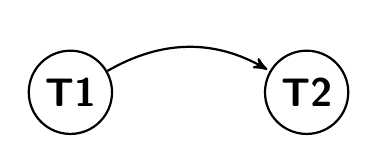
\begin{tikzpicture}[->,>=stealth',shorten >=1pt,auto,node distance=3cm,
		thick,main node/.style={circle,draw,font=\sffamily\Large\bfseries}]

	\node[main node] (T1) {T1};
	\node[main node] (T2) [right of=T1] {T2};

	\path[every node/.style={font=\sffamily\small}]
	(T1) edge [bend left] node {} (T2);

	\end{tikzpicture}
	\item Table \ref{table:1} shows the filled timestamp table. No TXN reset is concerned.

	\begin{table}[h!]
		\centering
		\begin{tabular}{|c|c|c|}
		\hline
		\textbf{Operation} & \textbf{R-TS(A)} & \textbf{W-TS(A)} \\ \hline
		\textbf{R1(A)}     & 1       & 0       \\ \hline
		\textbf{W1(A)}     & 1       & 1       \\ \hline
		\textbf{R2(A)}     & 2       & 1       \\ \hline
		\textbf{W2(A)}     & 2       & 2       \\ \hline
		\end{tabular}
		\caption{Q1}
		\label{table:1}
	\end{table}

\end{enumerate}

\section*{Problem 2}
\begin{enumerate}
	\item Table \ref{table:2}. W1 is ignored.
	\begin{table}[h!]
		\centering
		\begin{tabular}{|c|c|c|}
		\hline
		\textbf{Operation} & \textbf{R-TS(A)} & \textbf{W-TS(A)} \\ \hline
		\textbf{R1(A)}     & 1       & 0       \\ \hline
		\textbf{W2(A)}     & 1       & 2       \\ \hline
		\textbf{W1(A)}     & 1       & 2       \\ \hline
		\end{tabular}
		\caption{Q2}
		\label{table:2}
	\end{table}

	\item The definition of conflict requires that at least one operation is a write, which means there is only one pair on conflict in $S$. But here we have to show that $S$ is not serializable. I assume $R_1 (A)$ conflicts with $W_2 (A)$ and $W_2 (A)$ conflicts with $W_1 (A)$ so that its precedence graph has a cycle. $S$ is not serializable.
	\item For the schedule in (1), the serial schedule is $S' = R_1 (A),W_1 (A),W_2 (A)$. (i) The read is equivalent as it is the first operation. (ii) in both schedule, the last write is $W_2 (A)$. $S$ is view serializable.
\end{enumerate}

\section*{Problem 3}
For a already generated schedule, each TXN has a timestamp. Consider a serial schedule useing this timestamp as sequence.

(i) The basic read rules ensure that for any certain read in ant TXN would happen after all the write on the same item that take place before this TXN, becasue $TS(T)>=TS-W(A)$. Also, according to the potocal, the most recent write on this item should not be ignored for a write with larger timestamp must appear after this read. This ensures this read is equivalent to the read in the serial schedule.

(ii) The final write of an item in the serial schedule is done by the TXN that write on this item with largest timestamp. In the generated schedule, this write operation has the largest timestamp and will not be ignored. All other write before this can be ignored, but that do not matter. The final write is from the same TXN. 

\section*{Problem 4}
\begin{tcolorbox}[colback=gray!10, breakable]
	How long does it take you to finish the assignment? Give a score (1,2,3,4,5) to the difficulty of each problem. List all your collaborators if you have any.
\end{tcolorbox}
Done during first round rewiew. Within one hour. 2, 2, 4.
\end{document}